%%%%%%%%%%%%%%%%%%%%%%%%%%%%%%%%%%%%%%%%%%%%%%%%%%%%%%%%%%%%%%%%%%%%%%%%
%                                                                      %
%     File: Thesis_Implementation.tex                                  %
%     Tex Master: Thesis.tex                                           %
%                                                                      %
%     Author: Andre C. Marta                                           %
%     Last modified :  2 Jul 2015                                      %
%                                                                      %
%%%%%%%%%%%%%%%%%%%%%%%%%%%%%%%%%%%%%%%%%%%%%%%%%%%%%%%%%%%%%%%%%%%%%%%%

\chapter{Solution}
\label{chapter:implementation}

In the current chapter we detail our approach to construct a machine learning model that detects malware based on static and dynamic features, as well as practicals applications of such model.

We first define how the training data was collected and analyzed, followed by how it was labeled.
Having the data labeled, we detail what features were used for the machine learning model, based on the available data. We then explain the used model that learned to detect malware based on the selected features, its advantages and disadvantages. To measure how well the model fitted the data we describe how the evaluation was made, with special attention on keeping temporal consistent evaluations (i.e.\ training samples predates validation samples). We close the chapter with how we applied our model in a real-world scenario, as to enhance the credibility and usability of the main subject: malware detection via machine learning.

%%%%%%%%%%%%%%%%%%%%%%%%%%%%%%%%%%%%%%%%%%%%%%%%%%%%%%%%%%%%%%%%%%%%%%%%
\section{Data Sources}
\label{section:data_sources}

The purpose of this step is to obtain a corpus from which information
about malware and goodware can be extracted.
To minimize any possible bias towards data collection, and to save the overhead time of collecting and analyzing samples, we chose to take advantage of the publicly available reports from \textcolor{red}{Malwr} service.
As previously mentioned in \textcolor{red}{malwr cuckoo section}, Malwr is a free online service that does static and dynamic analysis on submitted files using \textcolor{red}{Cuckoo}, which are then accessible in an HTML report.

Our first approach was to apply a common data extraction technique, where online data is saved locally or in a central database for further analysis, to the list of analysis in Malwr\footnote{Malwr Analysis list [https://malwr.com/analysis/]}.
This technique, called \textit{scraping}, was done using \textcolor{red}{Scrapy}, a Python scraping library.
It is worth noting this scraping did not provide us the full analysis report, only information regarding the type of submission (e.g. binary, text, archive), its submission date and the sample MD5 hash.
After narrowing down the type of submissions, we applied a second scraping to Malwr, in order to obtain the full HTML reports. In Section \ref{section:data_analysis} we detail on how we narrowed the type of submissions.

To enrich our knowledge about samples' \textit{ground truth} we resorted to two other online repositories: \textcolor{red}{National Software Reference Library (NSRL)} and \textcolor{red}{VirusShare.com}, these provide metadata (e.g. MD5 hash) regarding known goodware and malware samples, respectively.
As \textcolor{red}{NSRL} contains a collection of digital signatures of known, traceable software applications, if a sample is present in this collection, we are more confident it is indeed goodware.
On the other hand, VirusShare.com is a repository of malware samples, hence a sample present in this repository gives us a higher confidence it is indeed malware.

%%%%%%%%%%%%%%%%%%%%%%%%%%%%%%%%%%%%%%%%%%%%%%%%%%%%%%%%%%%%%%%%%%%%%%%%
\section{Data Analysis}
\label{section:data_analysis}

After our initial scraping to obtain a high level view of the available reports, we observed that \textcolor{red}{Malwr} had a total of 642,698 submissions, dated between April 16th, 2013 and October 10th, 2016. As can be seen in Figure \ref{fig:samples_count}, there was an increase in sample submission from 2013 up to all time highs in May, June and July of 2014, followed by possibly a downtime period in August 2014.
The service went back up in September 2014, after which it stabilized around 20,000 submissions per month.

\begin{figure}[!htb]
	\centering
	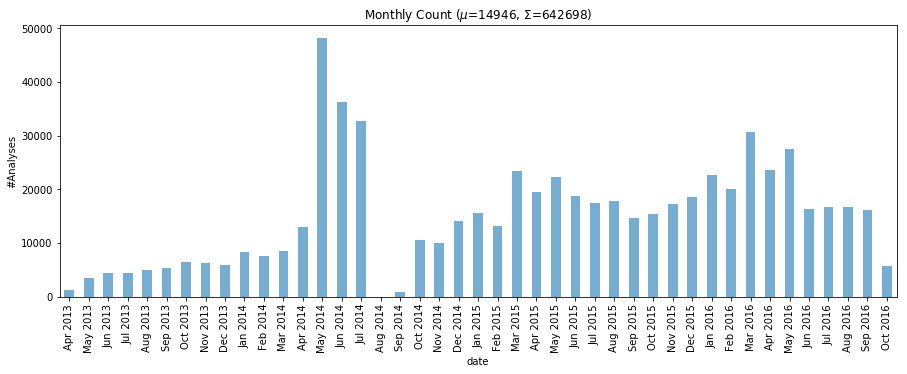
\includegraphics[width=0.95\textwidth]{Figures/samples_count.png}
	\caption[Number of monthly submissions.]{Number of monthly submissions.}
	\label{fig:samples_count}
\end{figure}

Followed this initial observation, we measured the percentage of duplicated submissions per month, which vary between 10\% and 20\%, and the percentage of different file types, as shown in Figure \ref{fig:monthly_distributions}.
The file types distribution is interesting, as it shows that executables (i.e.\ compiled binary files) took the great majority of submissions up to the end of 2014, after which documents (e.g.\ Word, Excel) and text files (e.g.\ HTML, JavaScript) started to increase.
As a side observation, this increase might indicate how users are more suspicious of these type of files, given that it is not uncommon to see malware being distributed in documents (under email attachments) and in websites (as JavaScript scripts) in more recent years.

\begin{figure}[!htb]
	\begin{subfigmatrix}{2}
		\subfigure[Percentage of duplicated submissions per month (based on MD5).]{\includegraphics[width=0.95\linewidth]{Figures/samples_dups.png}}
		\subfigure[Distribution of file types per month.]{\includegraphics[width=0.95\linewidth]{Figures/samples_types.png}}
	\end{subfigmatrix}
	\caption[Monthly distributions of submissions.]{Monthly distributions of submissions.}
	\label{fig:monthly_distributions}
\end{figure}

Having a better overall understanding on the available reports, and taking into account the limitations of static analysis in \textcolor{red}{Cuckoo} as mentioned in \textcolor{red}{malwr cuckoo section}, led us to our first data selection criteria: collect reports from \textcolor{red}{PE} (e.g.\ 32bit executables, DLL's) submissions only.
This selection reduces the number of available reports to 388,702 (60.48\% of the total) but enables us to work with more static information.

We went on to extract these reports, again using \textcolor{red}{Scrapy}, as HTML files and kept them in a gzip compressed format to save disk space.
A set $\mathcal{R}$ of raw reports, totaling 388,507 submissions was obtained, (different from the
previous amount as some errors could have occurred during scraping) occupying a total of 26GB.

As previously mentioned in \textcolor{red}{malwr cuckoo section}, Malwr aggregates the scan report as provided by VirusTotal, which entails multiple antivirus classifications.
Our next analysis takes advantage of this information to better understand how the samples are labeled and how reliable using the VirusTotal report can be to label our dataset.

We started by creating a set $\mathcal{C}\subseteq\mathcal{R}$ of 284,880 classified reports.
This set was achieved by selecting vendors that were present in at least 95\% of the classified reports, as to guarantee that vendors did not show occasionally.
The selected vendors $\mathcal{V}$ total to 37, out of 97 that appear at least once in a report.


Our next analysis was to understand how each sample was classified by different vendors.



%\begin{figure}[!htb]
%	\subfloat[Total samples per month]{
%		\includegraphics[width=0.95\textwidth]{samples_dups.png}
%	}\\
%	\subfloat[Percentage of duplicated (same MD5) samples per month]{
%		\includegraphics[width=0.95\textwidth]{samples_types.png}
%	}
%	\caption{Statistics for the scraped submissions. Count and percentage of duplicates}
%	\label{fig:dist_submissions}
%\end{figure}

\newpage

Description of the numerical implementation of the models explained in Chapter~\ref{chapter:background}...

%%%%%%%%%%%%%%%%%%%%%%%%%%%%%%%%%%%%%%%%%%%%%%%%%%%%%%%%%%%%%%%%%%%%%%%%
\section{Data labeling}
\label{section:data_labeling}

%%%%%%%%%%%%%%%%%%%%%%%%%%%%%%%%%%%%%%%%%%%%%%%%%%%%%%%%%%%%%%%%%%%%%%%%
\section{Feature Selection}
\label{section:feature_selection}

%%%%%%%%%%%%%%%%%%%%%%%%%%%%%%%%%%%%%%%%%%%%%%%%%%%%%%%%%%%%%%%%%%%%%%%%
\section{Model Selection}
\label{section:model_selection}

%%%%%%%%%%%%%%%%%%%%%%%%%%%%%%%%%%%%%%%%%%%%%%%%%%%%%%%%%%%%%%%%%%%%%%%%
\section{Evaluation}
\label{section:evaluation}

%%%%%%%%%%%%%%%%%%%%%%%%%%%%%%%%%%%%%%%%%%%%%%%%%%%%%%%%%%%%%%%%%%%%%%%%
\section{Practical Applications}
\label{section:practical_applications}
